\documentclass[default]{beamer}
\setbeamertemplate{navigation symbols}{}

\usetheme{CambridgeUS}
\useoutertheme{infolines}
%\usecolortheme{crane}

\usepackage[utf8]{inputenc}					% Выбор языка и кодировки
\usepackage{csquotes}
\usepackage{tikz}
\usetikzlibrary{arrows,shapes,calc}
\usepackage{animate}
\usepackage{fp}
\usepackage{textpos}

\usepackage[
	language=auto,
	autolang=other,
	backend=biber,
	style=authortitle,
	sorting=ydnt,
	maxbibnames=5
]{biblatex}
\addbibresource{panov-bica.bib}
				
\DeclareSourcemap{
	\maps[datatype=bibtex, overwrite]{
		\map{
			\step[fieldset=langid, fieldvalue=english]
			\step[fieldset=doi, null]
			\step[fieldset=issn, null]
			\step[fieldset=isbn, null]
			\step[fieldset=url, null]
			\step[fieldsource=language, fieldset=langid, origfieldval]
		}
	}
}
\DeclareBibliographyDriver{std}{%
	\usebibmacro{bibindex}%
	\usebibmacro{begentry}%
	\usebibmacro{author/editor+others/translator+others}%
	\setunit{\labelnamepunct}\newblock
	\usebibmacro{title}%
	\newunit\newblock
	\usebibmacro{maintitle+booktitle}
	\newunit\newblock
	\usebibmacro{journal}%
	\newunit\newblock
	\usebibmacro{date}%
	\newunit\newblock
	\usebibmacro{finentry}
}
\DeclareBibliographyAlias{article}{std}
\DeclareBibliographyAlias{book}{std}
\DeclareBibliographyAlias{inproceedings}{std}
\DeclareBibliographyAlias{incollection}{std}

\graphicspath{{../../images/}} 			% Пути к изображениям

\makeatletter
\setbeamertemplate{footline}
{
	\leavevmode%
	\hbox{%
		\begin{beamercolorbox}[wd=.333333\paperwidth,ht=2.25ex,dp=1ex,center]{author
				in head/foot}%
			\usebeamerfont{author in
				head/foot}\insertshortauthor~~\beamer@ifempty{\insertshortinstitute}{}{(\insertshortinstitute)}
		\end{beamercolorbox}%
		\begin{beamercolorbox}[wd=.333333\paperwidth,ht=2.25ex,dp=1ex,center]{title in
				head/foot}%
			\usebeamerfont{title in head/foot}\insertshorttitle
		\end{beamercolorbox}%
		\begin{beamercolorbox}[wd=.333333\paperwidth,ht=2.25ex,dp=1ex,right]{date in
				head/foot}%
			\usebeamerfont{date in head/foot}\insertshortdate{}\hspace*{2em}
			\insertframenumber{}\hspace*{2ex} 
		\end{beamercolorbox}
	}%
	\vskip0pt%
}

\addtobeamertemplate{frametitle}{}{
	\begin{textblock*}{100mm}(\textwidth-35pt,-20pt)
		
\includegraphics[width=1.5cm]{advert/ras_en.png}
	\end{textblock*}
}

\newcommand{\predmatr}[3]{
	\node[ell, rectangle, minimum height = 15, minimum width = 7.5]  at (#1 pt,#2 pt) {}; 
	\node[ellf, rectangle, minimum height = 15, minimum width = 7.5] at (#1+7.5 pt,#2 pt) {};
	\node[minimum height = 15, minimum width = 15] (#3) at (#1+3.3pt,#2 pt) {};
	\draw[ell] (#1+7.5 pt,#2+7.5 pt) -- (#1 +7.5 pt,#2-7.5 pt);
}
\renewcommand*{\bibfont}{\tiny}
\setlength\bibitemsep{-5pt}

\begin{document}
	
	\title[Psychologically inspired planning]{Psychologically inspired planning method for smart relocation task}
	\author[Panov \& Yakovlev]{Aleksandr Panov and Konstantin Yakovlev}
	\institute[RAS]{Federal Research Center ``Computer Science and Control''\\\textbf{Russian Academy of Sciences (RAS)\\Moscow}}
	\date{July 18 -- BICA 2016} 
	
	
	\begin{frame}
		\titlepage
		\centering
		
\includegraphics[width=100pt]{advert/ras_en.png} \hspace{10pt}
		
\includegraphics[width=80pt]{advert/frccsc.png}
	\end{frame}
	
	\section{Introduction}
	\subsection{Sign world model}
	
	\begin{frame}
		\frametitle{Knowledge representation: sign world model}
		\onslide<1->{
			{\footnotesize
				A component of knowledge representation is a sign:
				\begin{itemize}
					\item in sense of cultural-historical approach by L. Vygotsky,
					\item in sense of activity theory by A. Leontiev.
				\end{itemize}
			}
		}
		\onslide<2->{
			\begin{columns}
				\begin{column}{0.4\textwidth}
					\centering
					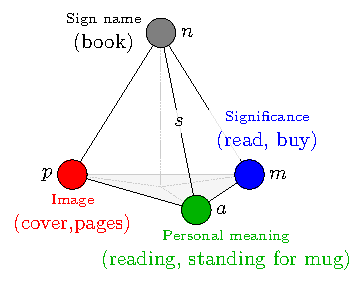
\includegraphics[width=0.7\textwidth]{signs/en/sign_colored_rita}
				\end{column}
				
		}
		\onslide<3->{
				\begin{column}{0.6\textwidth}
					\centering
					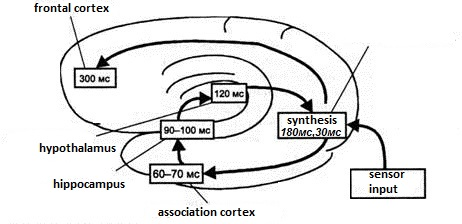
\includegraphics[width=0.6\textwidth]{phisio/ivan_cyrc_en}
				\end{column}
			\end{columns}
		
		
			{\footnotesize
				Supported ideas in psychology and biology:
				\begin{itemize}
					\item neurophysiological data (Edelman, Ivanitsky, Mountcastle etc.),
					\item two and three levels psychological theories (Stanovich, Kahneman).
				\end{itemize}
			}
			\vspace{-5pt}
			\nocite{*}
			\printbibliography[keyword={sign}, resetnumbers=true]
		}
	\end{frame}
	
	\begin{frame}
		\frametitle{Three constituents of knowledge}
		
		\begin{figure}
			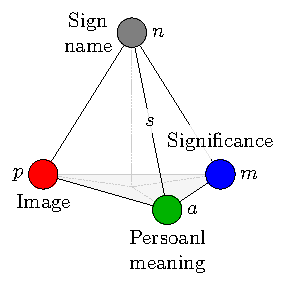
\includegraphics[width=0.3\textwidth]{signs/en/sign_colored_en}
		\end{figure}
		
		Mediated entity is represented with three causal structures:
		\begin{itemize}
			\item {\color{red}structure of image} - knowledge about external causal relations in input data,
			\item {\color{blue}structure of significance} - abstract generalized knowledge accumulated in culture,
			\item {\color{green!60!black}structure of personal meaning} - embodied knowledge including personal facilities, characteristics and motives.
		\end{itemize}
	\end{frame}

	\section{Sign grounding}
	\subsection{Neural substrate}
	\begin{frame}
		\frametitle{Neural substrate}
		
		\begin{columns}
			\begin{column}{0.35\textwidth}
				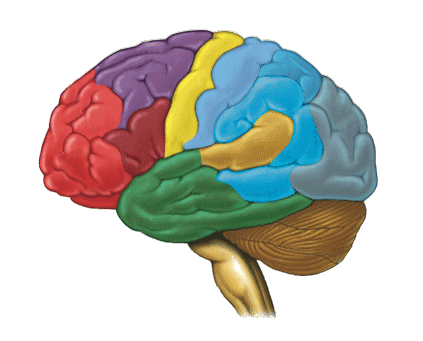
\includegraphics[width=0.8\textwidth]{phisio/mozg_2}
				\par\bigskip
				\hspace{-7mm}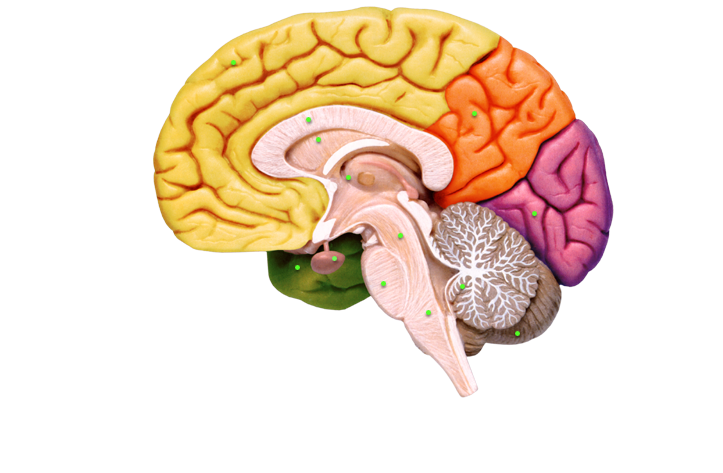
\includegraphics[width=\textwidth]{phisio/mozg}
			\end{column}
			\begin{column}{0.65\textwidth}
				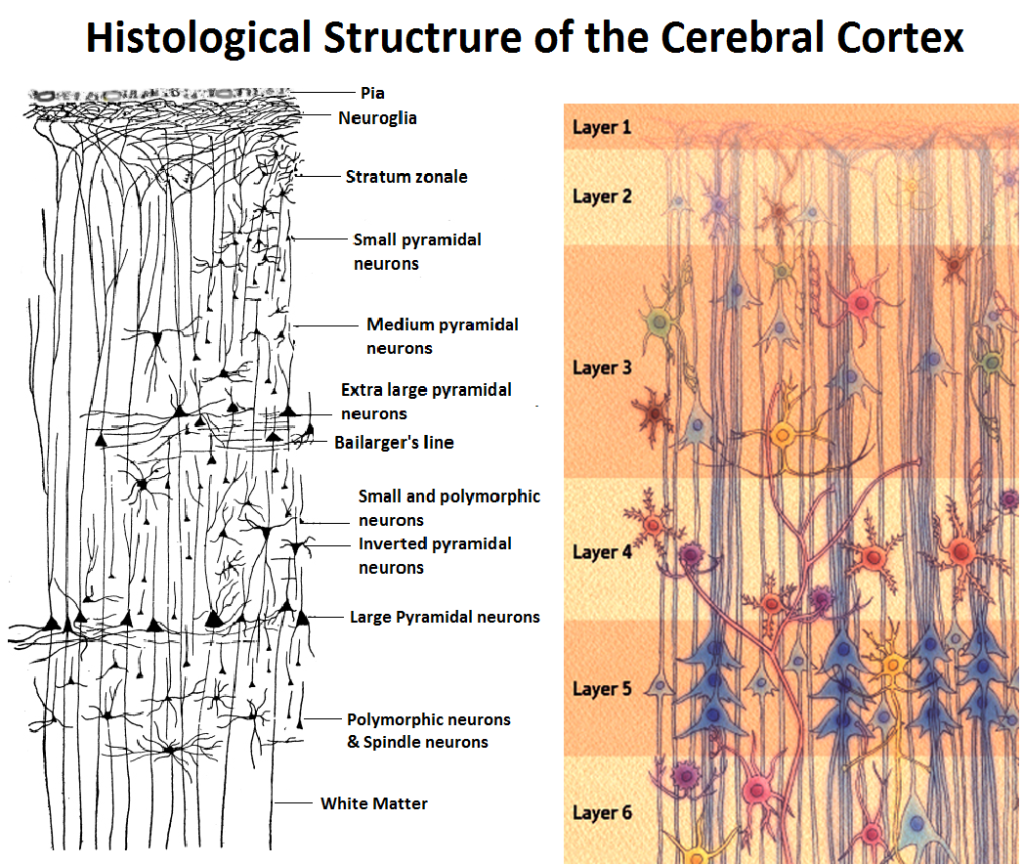
\includegraphics[width=\textwidth]{phisio/cortex_layers}
			\end{column}
		\end{columns}
		\nocite{*}
		\printbibliography[keyword={column}, resetnumbers=true]
	\end{frame}
	
	\begin{frame}
		\frametitle{Hierarchical model}
		
		Extended implementation of hierarchical temporal memory - \textbf{heterarchical causal framework}.
		\begin{overlayarea}{\textwidth}{\textheight}
			\only<1>{
				\begin{center}
					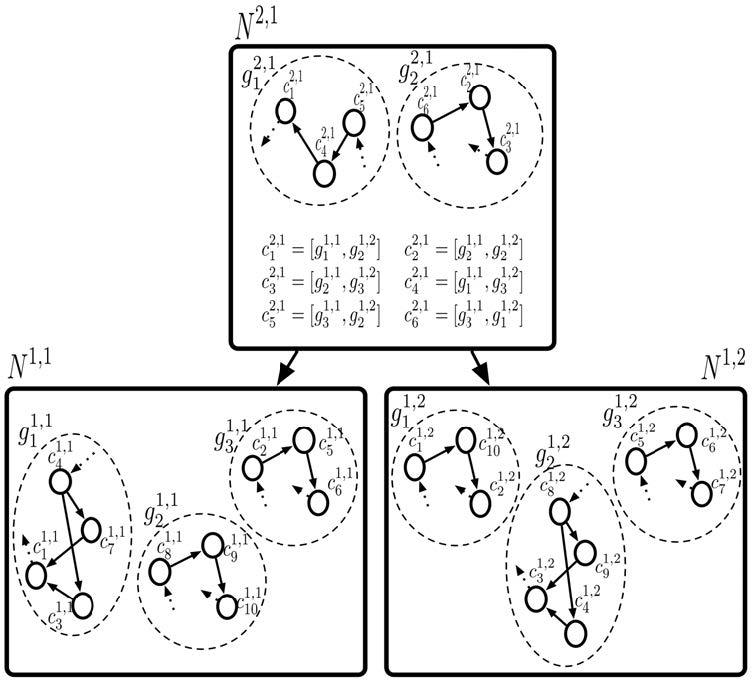
\includegraphics[width=0.6\textwidth]{mpf/hawkins_htm}
				\end{center}
			}
			\only<2>{
				\vspace{10pt}
				\centering
				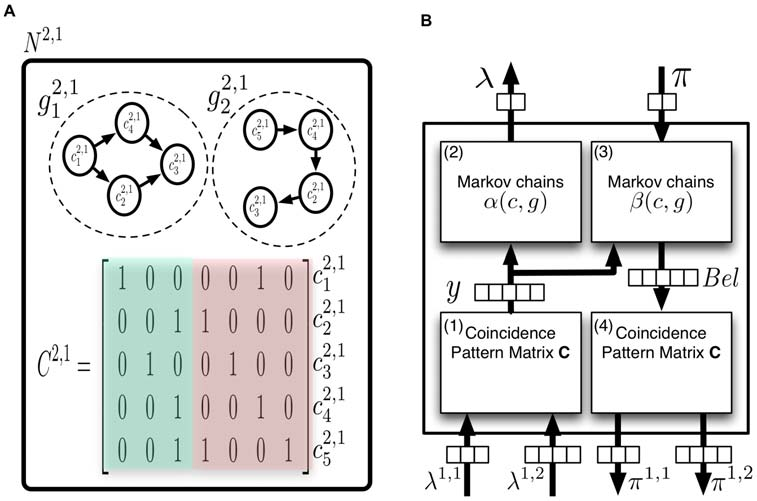
\includegraphics[width=0.6\textwidth]{mpf/hawkins_htm_ex}
			}
		\end{overlayarea}
	\end{frame}
	
	\begin{frame}
		\frametitle{Neuronal organization}
		
		\begin{columns}
			\begin{column}{0.65\textwidth}
				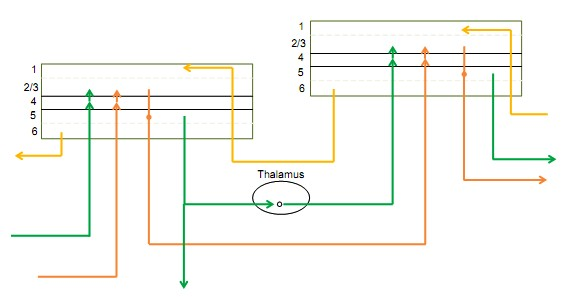
\includegraphics[width=0.9\textwidth]{mpf/regions_connect}
			\end{column}
			\begin{column}{0.35\textwidth}
				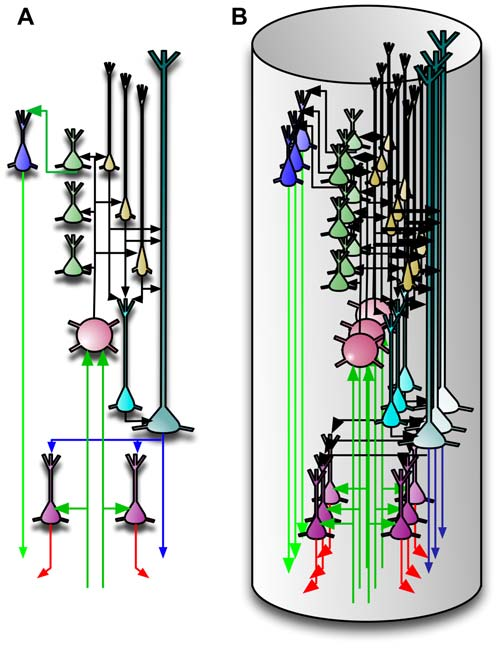
\includegraphics[width=\textwidth]{phisio/column}
			\end{column}
		\end{columns}
	\end{frame}
	
	\subsection{Causal matrix}
	\begin{frame}
		\frametitle{Causal matrix}                             
		\centering
		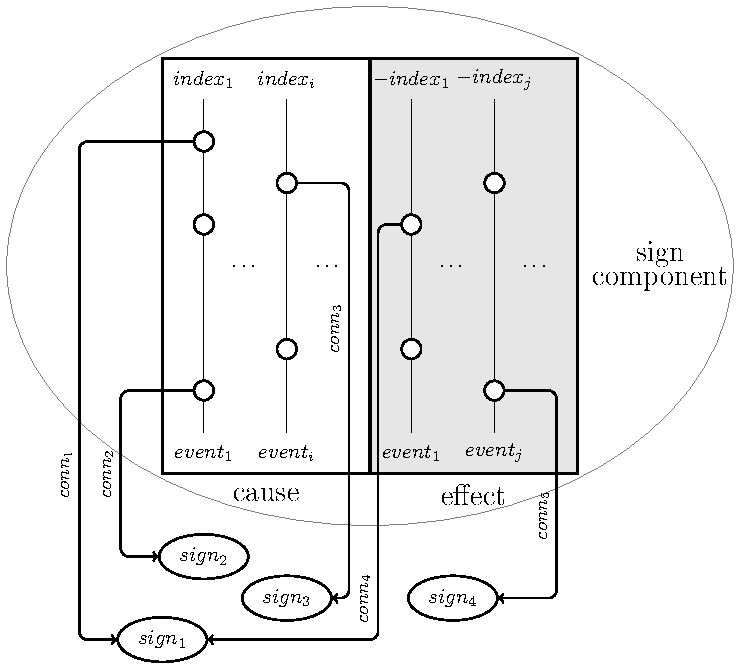
\includegraphics[width=0.7\textwidth]{automata/caus_matr}
		\vspace{10pt}
		\nocite{*}
		\printbibliography[keyword={per}, resetnumbers=true]
	\end{frame}

	\subsection{Perception model}	
	\begin{frame}
		\frametitle{Algorithm $\mathfrak A_{th}$ of sign component actualization}
		
		\begin{tikzpicture}[overlay,remember picture]
		
		\tikzstyle{z_matrix} = [draw, rectangle, minimum width = 60, minimum height = 60,fill=white];
		
		\onslide<1->{
			\node (meas_fun) at (0.7,0.5) {$\hat f_1,\hat f_2\dots,\hat f_k$};	
		}
		\onslide<2->{
			\node (control_vect) at ($(meas_fun)+(-0.5,1.2)$) {$\hat x^{j+1}$};
			\path[->,thick,red] (control_vect.east)  edge[out = -45, in = 45, right] (meas_fun.north); 
		}
		\onslide<3->{
			\node[z_matrix] (z_1) at ($(meas_fun)+(2.6,-0.5)$) {};
			\node[z_matrix] at ($(z_1)+(0.2,-0.1)$) {};
			\node[z_matrix] at ($(z_1)+(0.4,-0.2)$) {};
			
			\node[z_matrix] at ($(z_1)+(0.9,-0.5)$) {};
			\node[z_matrix] at ($(z_1)+(1.1,-0.6)$) {};
			\node[z_matrix] at ($(z_1)+(1.3,-0.7)$) {};
			
			\path[->,thick,blue] ([xshift=20]meas_fun.south)  edge[out = -90, in = -155, right] ($(z_1)+(-1,-1.2)$);
			\path[->,thick,blue] ([xshift=-25]meas_fun.south)  edge[out = -90, in = -155, right] ($(z_1)+(-0.1,-1.7)$);
			
			\node at ($(z_1)+(-1,1.4)$) {$Z^*$};
			
			\node at ($(z_1)+(0.8,1.4)$) {$Z_1$};
			\node at ($(z_1)+(1.4,1.2)$) {$\ddots$};
			\node at ($(z_1)+(2,0.9)$) {$Z_k$};
		}
		
		\onslide<4->{
			\draw[ultra thick, green!60!black] ($(z_1)+(-0.4,-1.1)$) -- ($(z_1)+(-0.4,0.6)$);
			\draw[ultra thick, green!60!black] ($(z_1)+(0.5,-1.6)$) -- node[right,black] {$z_1^r$} ($(z_1)+(0.5,0.1)$);
			
			\draw[->, thick, green!60!black] ($(z_1)+(-0.1,-3)$) -- node[right,black] {$\bar x(0)$} ($(z_1)+(-0.1,-2)$);
		}
		
		\onslide<5->{
			\node[z_matrix] (z_2) at ($(z_1)+(5,0)$) {};
			\node[z_matrix] at ($(z_2)+(0.2,-0.1)$) {};
			
			\node[z_matrix] at ($(z_2)+(0.9,-0.5)$) {};
			\node[z_matrix] at ($(z_2)+(1.3,-0.7)$) {};
			
			\node at ($(z_2)+(-1,1.4)$) {$Z^*$};
			\node at ($(z_2)+(0.8,1.4)$) {$Z_1$};
			\node at ($(z_2)+(1.4,1.2)$) {$\ddots$};
			\node at ($(z_2)+(2,0.9)$) {$Z_k$};
			
			\draw[->, ultra thick] ($(z_1)+(2.6,-0.6)$) -- node [above] {\scriptsize$\frac{\|\bar z_1^r-\bar x(0)\|}{\|\bar z_1^r\|+\|\bar x(0)\|}$} ($(z_1)+(3.7,-0.6)$);
			
			\draw[ultra thick, dotted, green!60!black] ($(z_2)+(-0.6,-1)$) -- ($(z_2)+(-0.6,0.7)$);
			\draw[ultra thick, dotted, green!60!black] ($(z_2)+(0.5,-1.6)$) -- ($(z_2)+(0.5,0.1)$);
		}
		
		\onslide<6->{
			\draw[->, thick, red] ($(z_2)+(0.3,1.4)$) -- node[right,black] {$\bar x^*(0)$} ($(z_2)+(0.3,3)$);
		}
		
		\onslide<7>{
			\draw[<-, thick, red] ($(z_2)+(-0.1,-3)$) -- node[right,black] {$\hat x^j(0)$} ($(z_2)+(-0.1,-2)$);
		}
		
		\onslide<7->{				
			\draw[ultra thick, green!60!black] ($(z_2)+(-0.4,-1)$) -- ($(z_2)+(-0.4,0.7)$);
			\draw[ultra thick, green!60!black] ($(z_2)+(0.7,-1.6)$) -- node[right,black] {$z_2^r$} ($(z_2)+(0.7,0.1)$);	
		}
		\onslide<8->{
			\draw[->, thick, green!60!black] ($(z_2)+(-0.1,-3)$) -- node[right,black] {$\bar x(1)$} ($(z_2)+(-0.1,-2)$);
		}
		
		\onslide<9->{
			\draw[->, ultra thick] ($(z_2)+(2.6,-0.6)$) -- node [above] {\scriptsize$\frac{\|\bar z_1^r-\bar x(1)\|}{\|\bar z_1^r\|+\|\bar x(1)\|}$} ($(z_2)+(3.7,-0.6)$);
		}
		\end{tikzpicture}
		
	\end{frame}	
			
	\begin{frame}
		\frametitle{Representation levels}
		
		\begin{figure}
			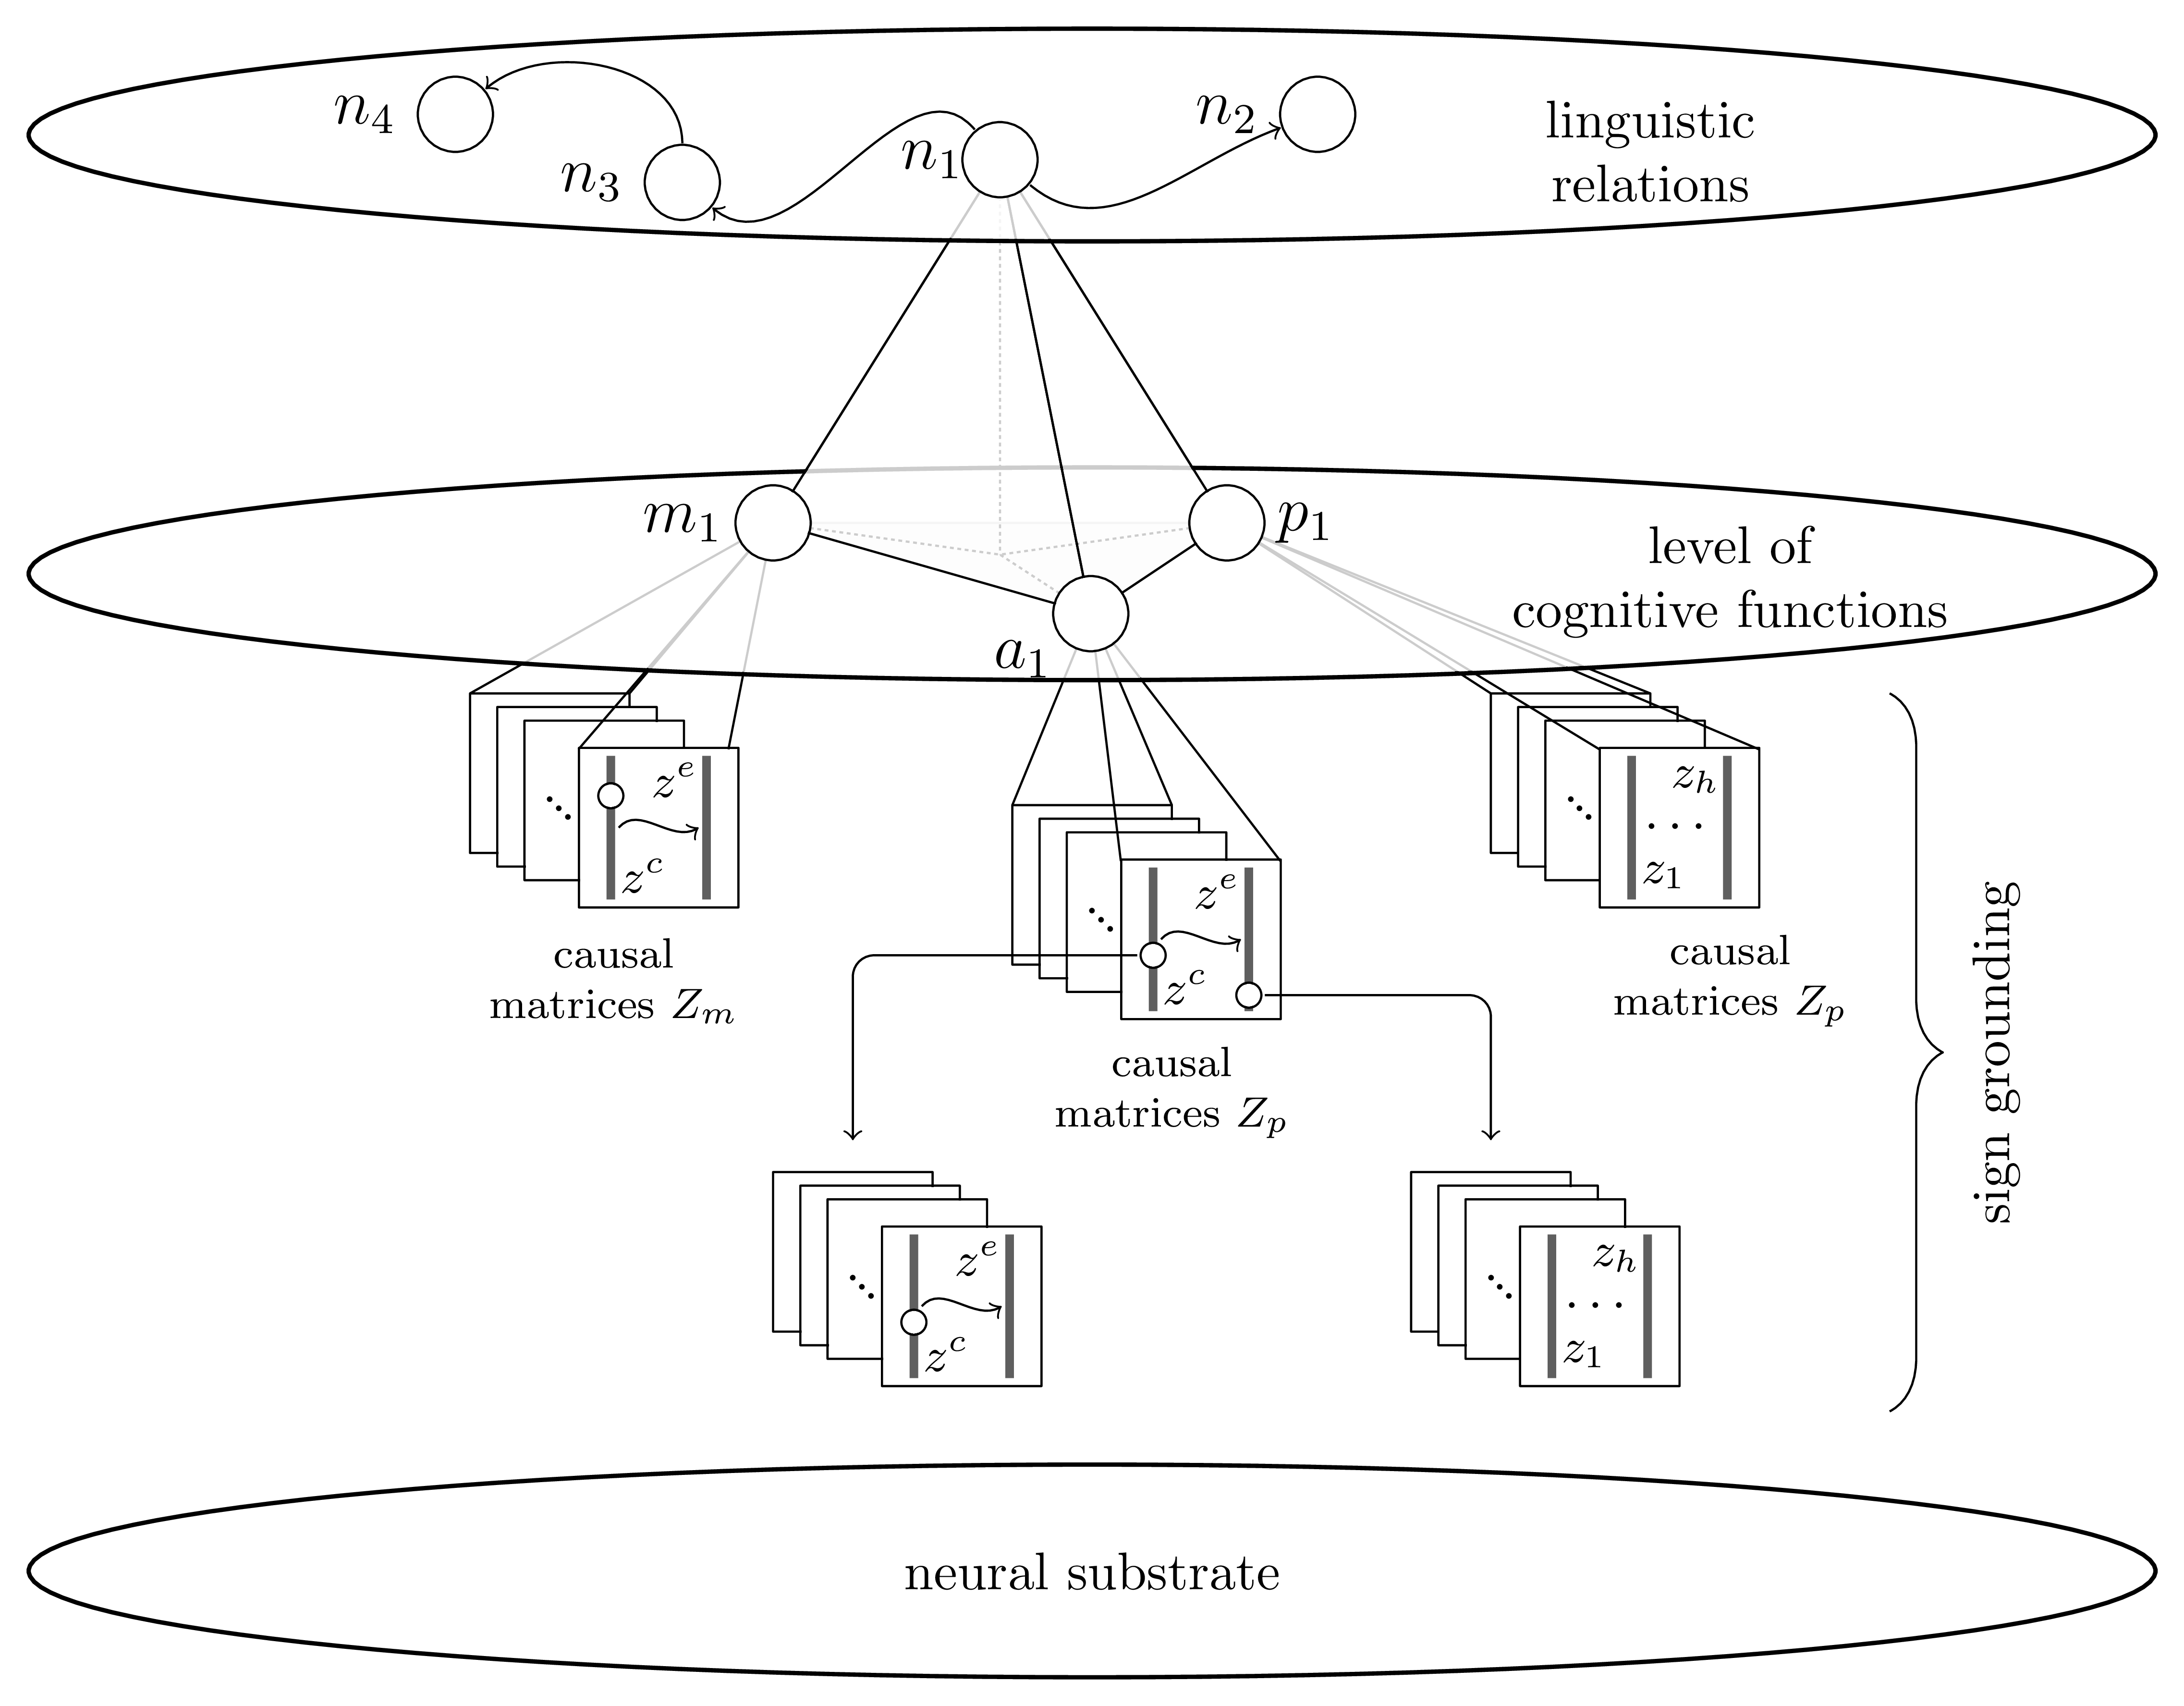
\includegraphics[width=0.7\textwidth]{signs/en/sign_levels_en}
		\end{figure}
	\end{frame}

	\section{Level of cognitive functions}
	\subsection{Semiotic network}
	\begin{frame}
		\frametitle{Sign world model}
		
		\begin{columns}
			\begin{column}{0.55\textwidth}
				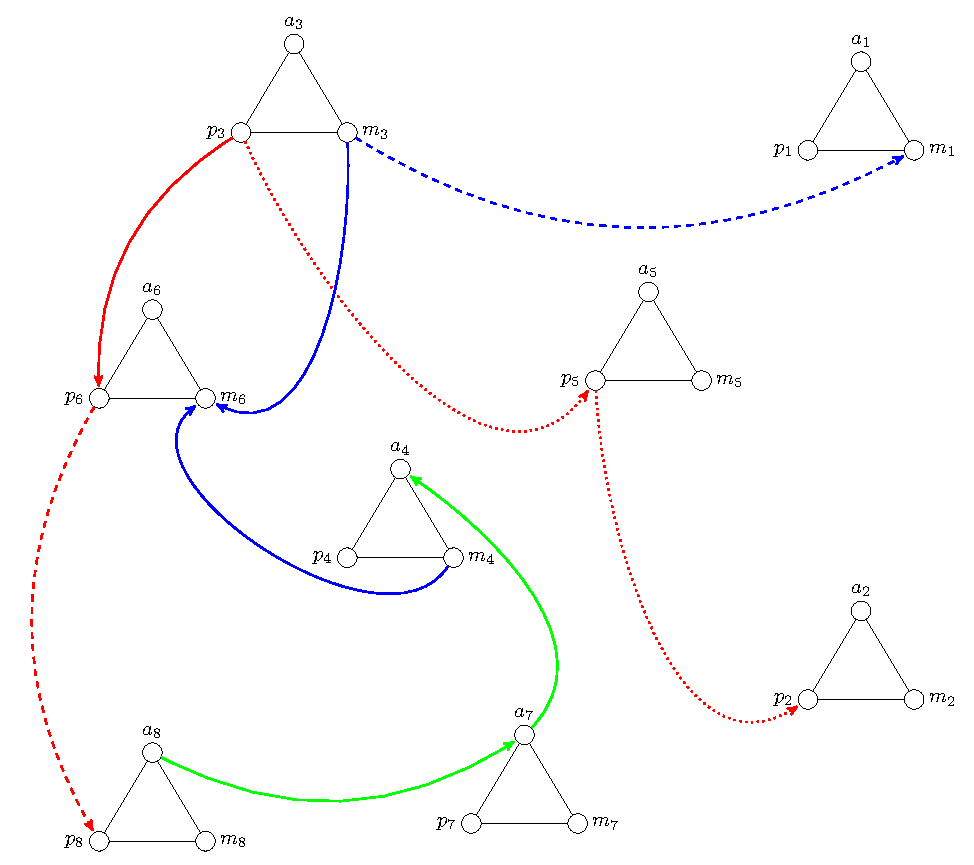
\includegraphics[width=\textwidth]{signs/signs_net}
			\end{column}
			\begin{column}{0.45\textwidth}
				\textit{Semiotic network} $H=\langle H_P, H_A, H_M\rangle$ consisting of three semantic network: 
				\begin{itemize}
					\item $H_P=\langle2^P,\mathfrak R_P\rangle$ -- semantic network on the set of sign images,
					\item $H_P=\langle2^A,\mathfrak R_A\rangle$ -- semantic network on the set of sign meanings,
					\item $H_P=\langle2^M,\mathfrak R_M\rangle$ -- semantic network on the set of sign significances.
				\end{itemize}

			\end{column}
		\end{columns}
		\vspace{10pt}
		\nocite{*}
		\printbibliography[keyword={symbsign}, resetnumbers=true]		
	\end{frame}	

	\section{Planning model}
	\subsection{Overview}
	\begin{frame}
		\frametitle{Behavior planning algorithm}
		
		\begin{columns}
			\begin{column}{0.6\textwidth}
				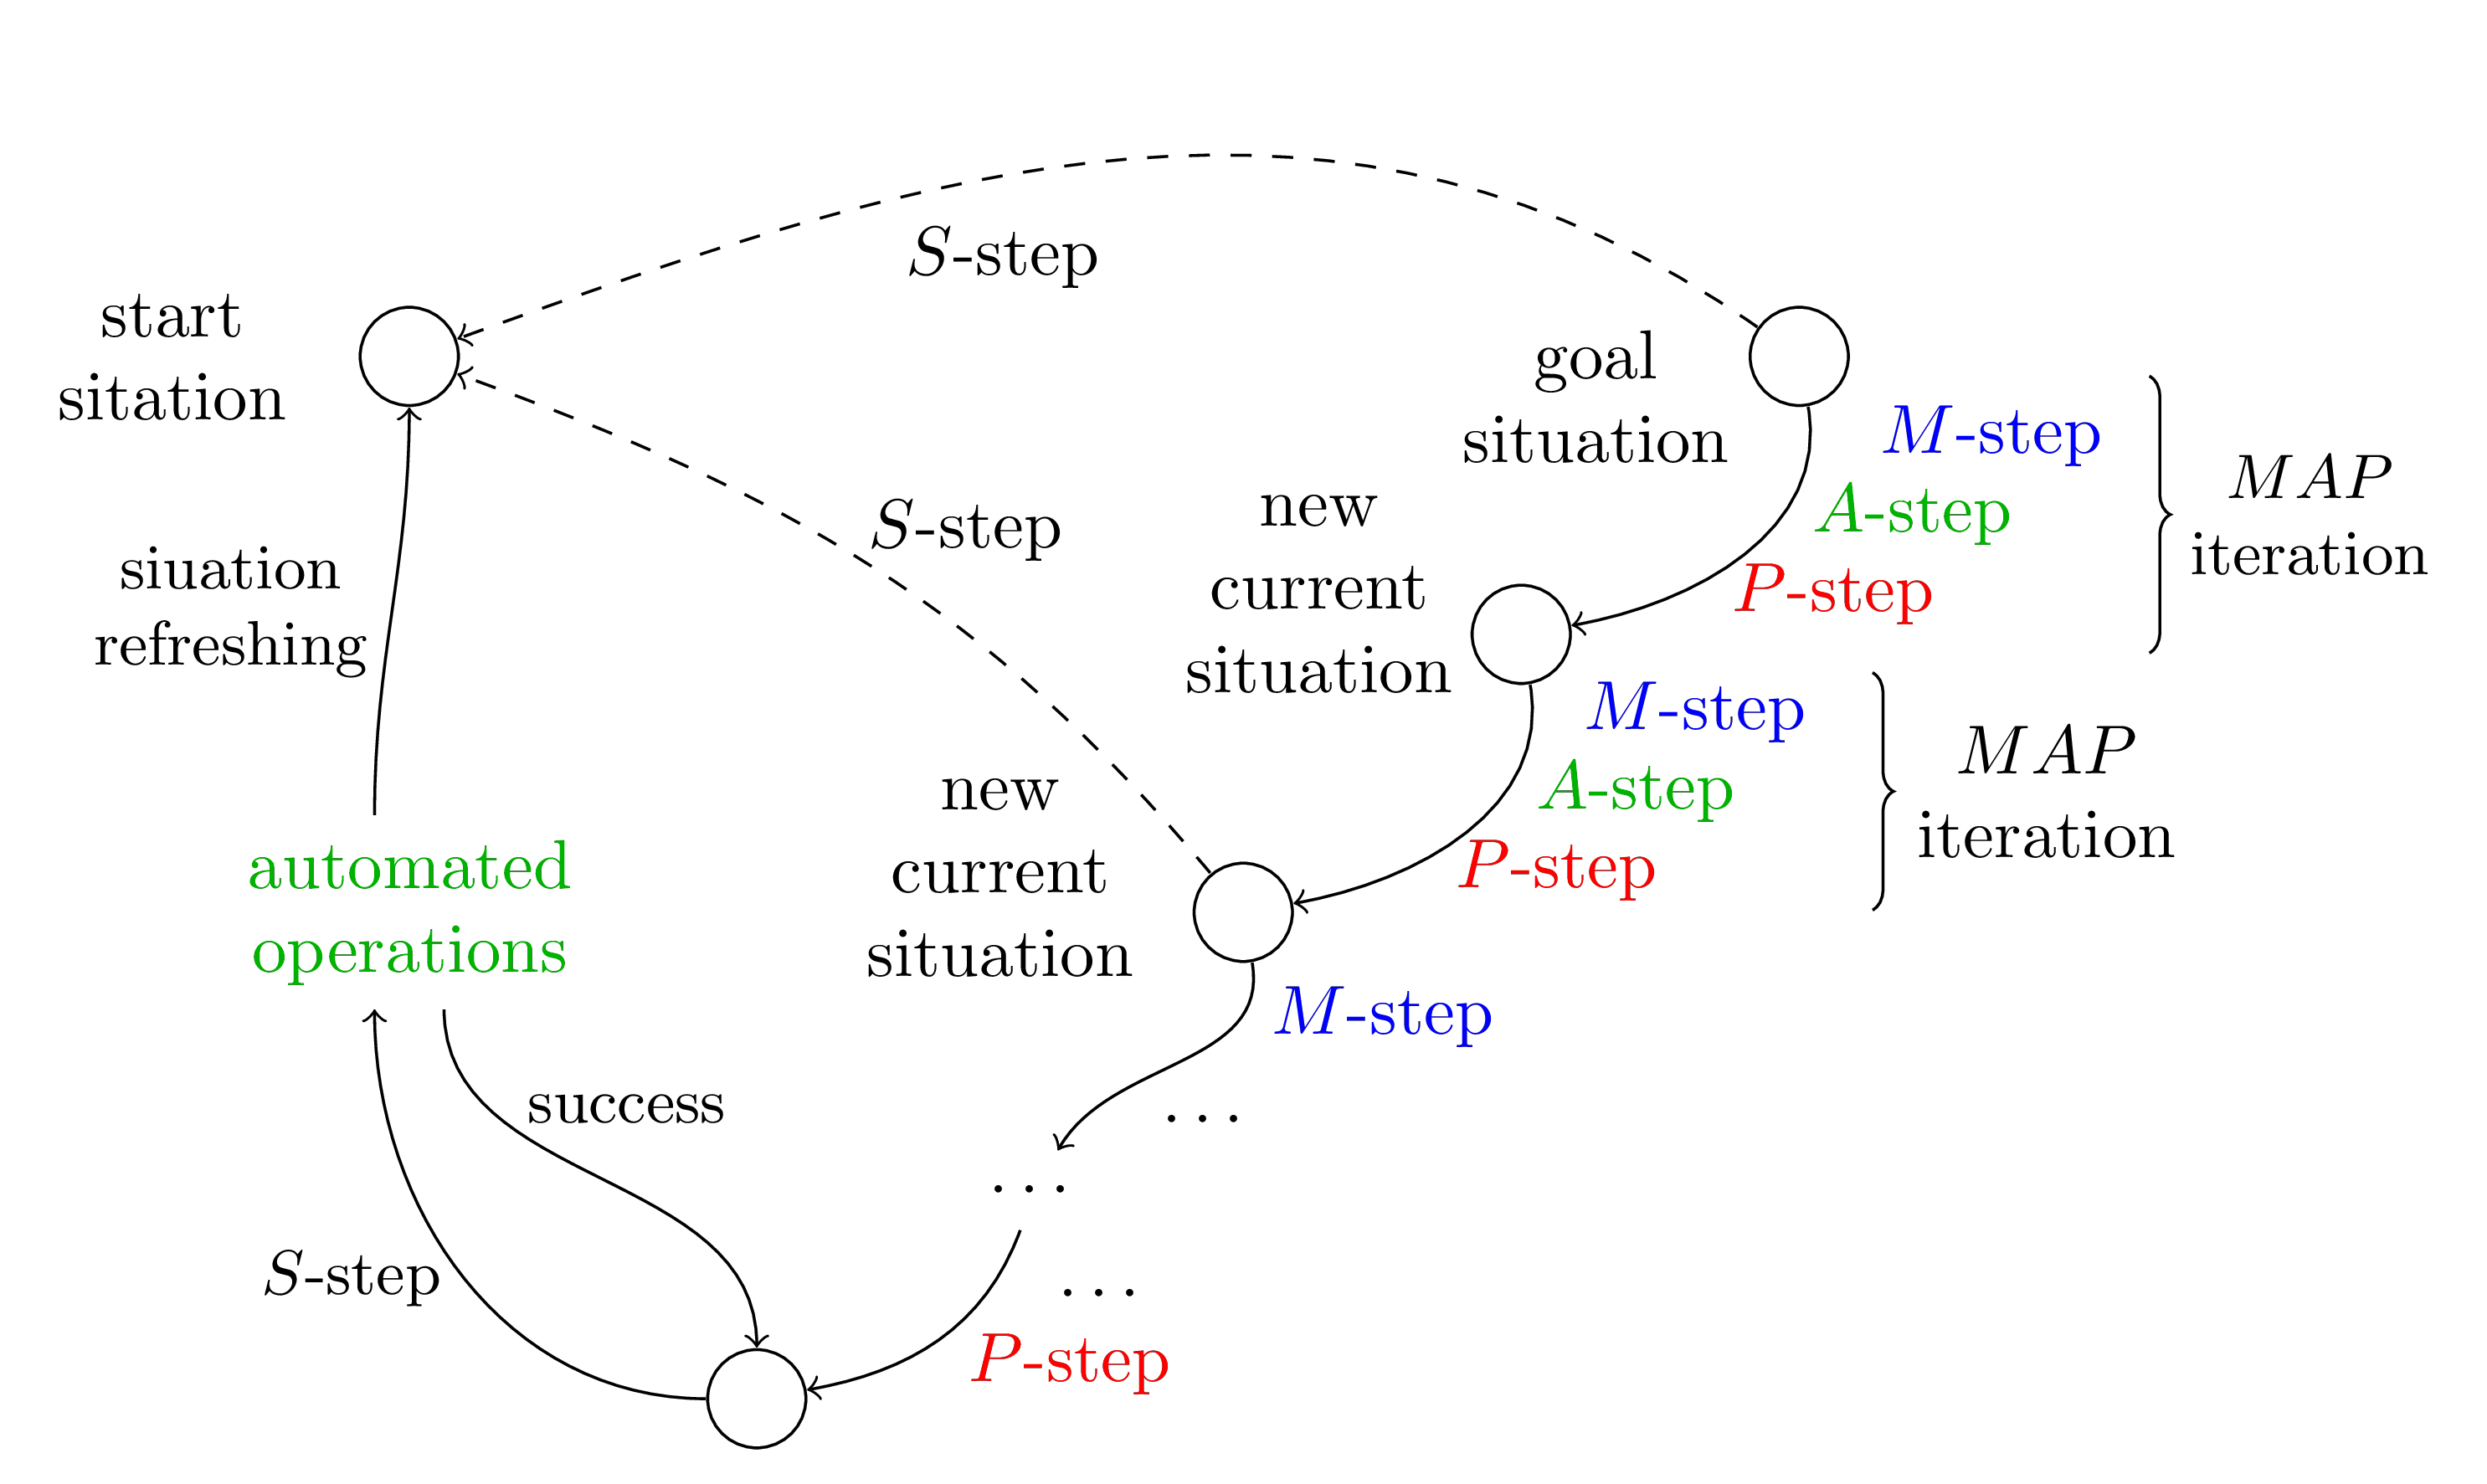
\includegraphics[width=\textwidth]{algo/en/beh_plan2_en}
				\vspace{10pt}
				\textbf{Key features}: hierarchical, online learning, meta-reasoning (heuristic generation), coalition support.
				\vspace{10pt}
				\nocite{*}
				\printbibliography[keyword={plan}, resetnumbers=true]
			\end{column}
			\begin{column}{0.4\textwidth}
				\scriptsize
				Planning starts from final situation and aims to meet start situation.
				\par\bigskip
				MAP iteration:
				\begin{itemize}
					\item \textit{M-step} -- search of relevant significances,
					\item \textit{A-step} -- choose a personal meaning from the set of personal meanings corresponding to the found significances,
					\item \textit{P-step} -- construct the new current situation using the set of features from the condition of performed action,
					\item \textit{S-step} -- send a message to other members of the coalition  or perform the action corresponding to the chosen personal meaning or execute action hierarchy up to \color{green!70!black} automated operations.
				\end{itemize}
			\end{column}
		\end{columns}
		
	\end{frame}	
	
	\subsection{Examples}
	\begin{frame}
		\frametitle{Example: fragment of network on significances}
		\begin{columns}
			\begin{column}{0.7\textwidth}
				\centering
				\includegraphics[page=2,width=\textwidth]{plan/plan_nets}
			\end{column}
			\begin{column}{0.3\textwidth}
				\centering
				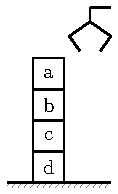
\includegraphics[page=1,width=\textwidth]{plan/block_world}
			\end{column}
		\end{columns}
	\end{frame}	
	
	\begin{frame}
		\frametitle{Example: network on meanings - start situation}
		
		\centering
		\includegraphics[page=3,width=0.7\textwidth]{plan/plan_nets}
		\par\bigskip
		\includegraphics[page=2,width=0.5\textwidth]{plan/block_world}
		
		
	\end{frame}	
	
	\begin{frame}
		\frametitle{Example: network on meanings - goal situation}
		\begin{columns}
			\begin{column}{0.7\textwidth}
				\centering
				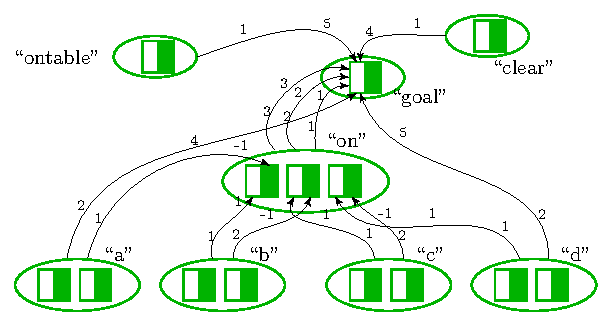
\includegraphics[page=1,width=\textwidth]{plan/plan_nets}
			\end{column}
			\begin{column}{0.3\textwidth}
				\centering
				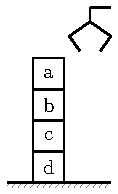
\includegraphics[page=1,width=\textwidth]{plan/block_world}
			\end{column}
		\end{columns}
	\end{frame}	
	
	\begin{frame}
		\frametitle{Example: fragment of network on significances}
		\begin{columns}
			\begin{column}{0.7\textwidth}
				\centering
				\includegraphics[page=5,width=\textwidth]{plan/plan_nets}
			\end{column}
			\begin{column}{0.3\textwidth}
				\centering
				\includegraphics[page=3,width=\textwidth]{plan/block_world}
			\end{column}
		\end{columns}
	\end{frame}
	
	\begin{frame}
		\frametitle{Example: generation of meanings}
		
		\begin{tikzpicture}[overlay,remember picture,xshift=165pt,yshift=-50pt]
		\onslide<1->{
			\tikzstyle{ell}=[draw, thick, align=center, color=blue]
			\tikzstyle{ellf}=[draw, thick, align=center, color=blue, fill=blue]
			
			\node[ell, ellipse, minimum height = 30, minimum width = 100] (block) at (5 pt,0){};
			\predmatr{-30}{0}{block1}
			\predmatr{-10}{0}{block2}
			\predmatr{10}{0}{block3}	
			\predmatr{30}{0}{block4}
			\node at (35 pt, 20 pt) {``block''};
			
			\node[ell, ellipse, minimum height = 20, minimum width = 40] (c) at (32.5 pt, -50 pt){};
			\predmatr{30}{-50}{c1}
			\node at (10 pt, -35 pt) {``c''};		
			
			\node[ell, ellipse, minimum height = 20, minimum width = 40] (d) at (82.5 pt, -50 pt){};
			\predmatr{80}{-50}{d1}			
			\node at (60 pt, -35 pt) {``d''};	
			
			\node[ell, ellipse, minimum height = 20, minimum width = 40] (x) at (-37.5 pt, 50 pt){};
			\predmatr{-40}{50}{x1}
			\node at (-85 pt, 50 pt) {``block?x''};			
			
			\node[ell, ellipse, minimum height = 20, minimum width = 40] (y) at (42.5 pt, 50 pt){};
			\predmatr{40}{50}{y1}	
			\node at (85 pt, 50 pt) {``block?y''};
			
			\path[-latex'] (c.north) edge [out = 90, in = -80] node[above, black] {\scriptsize 1} node[above, black, near start] {\scriptsize 1} ([xshift=-3]block3.south);
			\path[-latex'] (d.north) edge [out = 90, in = -80] node[above, black, near end] {\scriptsize 1} node[above, black, near start] {\scriptsize 1} ([xshift=-3]block4.south);	
		}
		\onslide<1>{
			\node[ell, ellipse, minimum height = 20, minimum width = 40] (a) at (-77.5 pt, -50 pt){};
			\predmatr{-80}{-50}{a1}
			\node at (-100 pt, -35 pt) {``a''};
			
			\node[ell, ellipse, minimum height = 20, minimum width = 40] (b) at (-27.5 pt, -50 pt){};
			\predmatr{-30}{-50}{b1}
			\node at (-50 pt, -35 pt) {``b''};		
		}
		\onslide<1-2>{
			\path[-latex'] (a.north) edge [out = 90, in = -120] node[above, black, near end] {\scriptsize 1} node[above, black, near start] {\scriptsize 1} ([xshift=-3]block1.south);
			\path[-latex'] (b.north) edge [out = 90, in = -120] node[above, black, near end] {\scriptsize 1} node[above, black, near start] {\scriptsize 1} ([xshift=-3]block2.south);
		}			
		\onslide<1-3>{
			\path[-latex'] ([xshift=-10]block.north) edge [out = 90, in = -80] node[above, black] {\scriptsize 1} node[above, black, near start] {\scriptsize 0} ([xshift=-3]x1.south);
			\path[-latex'] ([xshift=10]block.north) edge [out = 90, in = -100] node[above, black] {\scriptsize 1} node[above, black, near start] {\scriptsize 0} ([xshift=-3]y1.south);
		}
		\onslide<1-4>{
			\node[ell, ellipse, minimum height = 20, minimum width = 40] (unstack) at (2.5 pt, 100 pt){};
			\predmatr{0}{100}{unstack1}
			\node at (-15 pt, 120 pt) {``unstack''};
			
			\node[ell, ellipse, minimum height = 20, minimum width = 40] (on) at (-77.5 pt, 100 pt){};
			\predmatr{-80}{100}{on1}
			\node at (-115 pt, 100 pt) {``on''};
			
			\path[-latex'] (x.north) edge [out = 90, in = -100] node[above, black, near end] {\scriptsize -1} node[above, black, near start] {\scriptsize 1} ([xshift=2]unstack1.south);
			\path[-latex'] (y.north) edge [out = 90, in = -80] node[above, black, near end] {\scriptsize -2} node[above, black, near start] {\scriptsize 1} ([xshift=5]unstack1.south);
			\path[-latex'] (on.east) edge [out = 0, in = 180] node[above, black, near end] {\scriptsize 1} node[above, black, near start] {\scriptsize 1} ([yshift=-3]unstack1.west);
			
			\path[-latex'] ([xshift=-10]x.north) edge [out = 100, in = -140] node[above, black] {\scriptsize 1} node[above, black, very near start] {\scriptsize 1} ([xshift=-3]on1.south);	
			\path[-latex'] ([xshift=-10]y.north) edge [out = 150, in = -30] node[above, black, near end] {\scriptsize -1} node[above, black, very near start] {\scriptsize 1} ([xshift=3]on1.south);					
		}			
		\onslide<1-5>{
			\node[ell, ellipse, minimum height = 20, minimum width = 40] (holding) at (82.5 pt, 120 pt){};
			\predmatr{80}{120}{holding1}
			\node at (125 pt, 120 pt) {``holding''};
			
			\node[ell, ellipse, minimum height = 20, minimum width = 40] (clear) at (82.5 pt, 90 pt){};
			\predmatr{80}{90}{clear1}
			\node at (120 pt, 90 pt) {``clear''};
			
			\path[-latex'] (clear.west) edge [out = 180, in = 0] node[above, black, near end] {\scriptsize -2} node[above, black, near start] {\scriptsize 1} ([yshift=-3]unstack1.east);
			\path[-latex'] (holding.west) edge [out = 180, in = 0] node[above, black, near end] {\scriptsize -1} node[above, black, near start] {\scriptsize 1} ([yshift=3]unstack1.east);
			
		}
		\onslide<2->{
			\tikzstyle{ell}=[draw, thick, align=center, color=green!70!black]
			\tikzstyle{ellf}=[draw, thick, align=center, color=green!70!black, fill=green!70!black]
			
			\node[ell, ellipse, minimum height = 20, minimum width = 40] (a) at (-77.5 pt, -50 pt){};
			\predmatr{-80}{-50}{a1}
			\node at (-100 pt, -35 pt) {``a''};
			
			\node[ell, ellipse, minimum height = 20, minimum width = 40] (b) at (-27.5 pt, -50 pt){};
			\predmatr{-30}{-50}{b1}
			\node at (-50 pt, -35 pt) {``b''};
		}
		\onslide<3->{
			\path[-latex', very thick] (a.north) edge [out = 90, in = -120] node[above, black, near end] {\scriptsize 1} node[above, black, near start] {\scriptsize 1} ([xshift=-3]block1.south);
			\path[-latex', very thick] (b.north) edge [out = 90, in = -120] node[above, black, near end] {\scriptsize 1} node[above, black, near start] {\scriptsize 1} ([xshift=-3]block2.south);	
		}
		\onslide<4->{
			\path[-latex', very thick] ([xshift=-10]block.north) edge [out = 90, in = -80] node[above, black] {\scriptsize 1} node[above, black, near start] {\scriptsize 0} ([xshift=-3]x1.south);
			\path[-latex', very thick] ([xshift=10]block.north) edge [out = 90, in = -100] node[above, black] {\scriptsize 1} node[above, black, near start] {\scriptsize 0} ([xshift=-3]y1.south);
		}
		\onslide<5->{
			\node[ell, ellipse, minimum height = 20, minimum width = 40] (unstack) at (2.5 pt, 100 pt){};
			\predmatr{0}{100}{unstack1}
			\node at (-15 pt, 120 pt) {``unstack''};
			
			\node[ell, ellipse, minimum height = 20, minimum width = 40] (on) at (-77.5 pt, 100 pt){};
			\predmatr{-80}{100}{on1}
			\node at (-115 pt, 100 pt) {``on''};
			
			\path[-latex', very thick] (on.east) edge [out = 0, in = 180] node[above, black, near end] {\scriptsize 1} node[above, black, near start] {\scriptsize 1} ([yshift=-3]unstack1.west);
			
			\path[-latex', very thick] ([xshift=-10]x.north) edge [out = 100, in = -140] node[above, black] {\scriptsize 1} node[above, black, very near start] {\scriptsize 1} ([xshift=-3]on1.south);	
			\path[-latex', very thick] ([xshift=-10]y.north) edge [out = 150, in = -30] node[above, black, near end] {\scriptsize -1} node[above, black, very near start] {\scriptsize 1} ([xshift=3]on1.south);
			\path[-latex', very thick] (x.north) edge [out = 90, in = -100] node[above, black, near end] {\scriptsize -1} node[above, black, near start] {\scriptsize 1} ([xshift=2]unstack1.south);
			\path[-latex', very thick] (y.north) edge [out = 90, in = -80] node[above, black, near end] {\scriptsize -2} node[above, black, near start] {\scriptsize 1} ([xshift=5]unstack1.south);	
		}
		\onslide<6->{
			\node[ell, ellipse, minimum height = 20, minimum width = 40] (holding) at (82.5 pt, 120 pt){};
			\predmatr{80}{120}{holding1}
			\node at (125 pt, 120 pt) {``holding''};
			
			\node[ell, ellipse, minimum height = 20, minimum width = 40] (clear) at (82.5 pt, 90 pt){};
			\predmatr{80}{90}{clear1}
			\node at (120 pt, 90 pt) {``clear''};
			
			\path[-latex', very thick] (clear.west) edge [out = 180, in = 0] node[above, black, near end] {\scriptsize -2} node[above, black, near start] {\scriptsize 1} ([yshift=-3]unstack1.east);
			\path[-latex', very thick] (holding.west) edge [out = 180, in = 0] node[above, black, near end] {\scriptsize -1} node[above, black, near start] {\scriptsize 1} ([yshift=3]unstack1.east);
		}			
		\end{tikzpicture}
	\end{frame}
	
	\begin{frame}
		\frametitle{Example: meaning generation}
		\begin{columns}
			\begin{column}{0.7\textwidth}
				\centering
				\includegraphics[page=4,width=\textwidth]{plan/plan_nets}
			\end{column}
			\begin{column}{0.3\textwidth}
				\centering
				\includegraphics[page=3,width=\textwidth]{plan/block_world}
			\end{column}
		\end{columns}
	\end{frame}

	\begin{frame}
		\frametitle{Smart Relocation Tasks (SRT)}
		
		\begin{columns}
			\begin{column}{0.55\textwidth}
				\begin{center}
					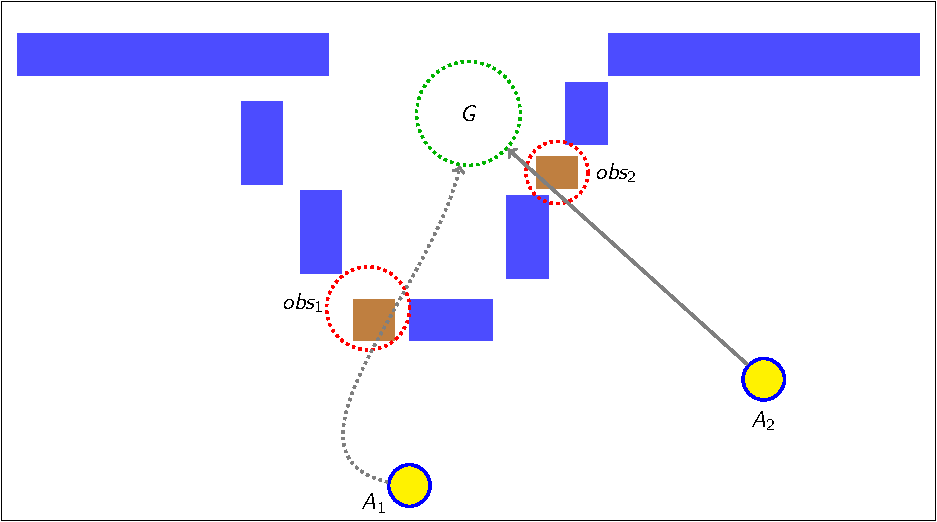
\includegraphics[page=1,width=0.85\textwidth]{examples/slides_colored}
				\end{center}
				
				\textbf{Problem}
				
				Goal area can not be achieved by some agents on their own (using standalone task and path planning methods)
				
				\textbf{Solution}
				
				Agents must communicate and some agents must alter their ``selfish'' plans in order to construct coalition plan
				
			\end{column}
			\begin{column}{0.45\textwidth}
				3 levels of control:
				\begin{itemize}
					\item Transformable environment
					\item Different types of obstacles (some -- can be destroyed)
					\item Agents with different capabilities (some agents can destroy obstacles, others -- can not)
					\item Common spatial goal (ALL agents must reach this region in order goal to be achieved)
				\end{itemize}
			\end{column}
		\end{columns}
	\end{frame}
	
	\begin{frame}
		\frametitle{Model task}
		
		\begin{figure}
			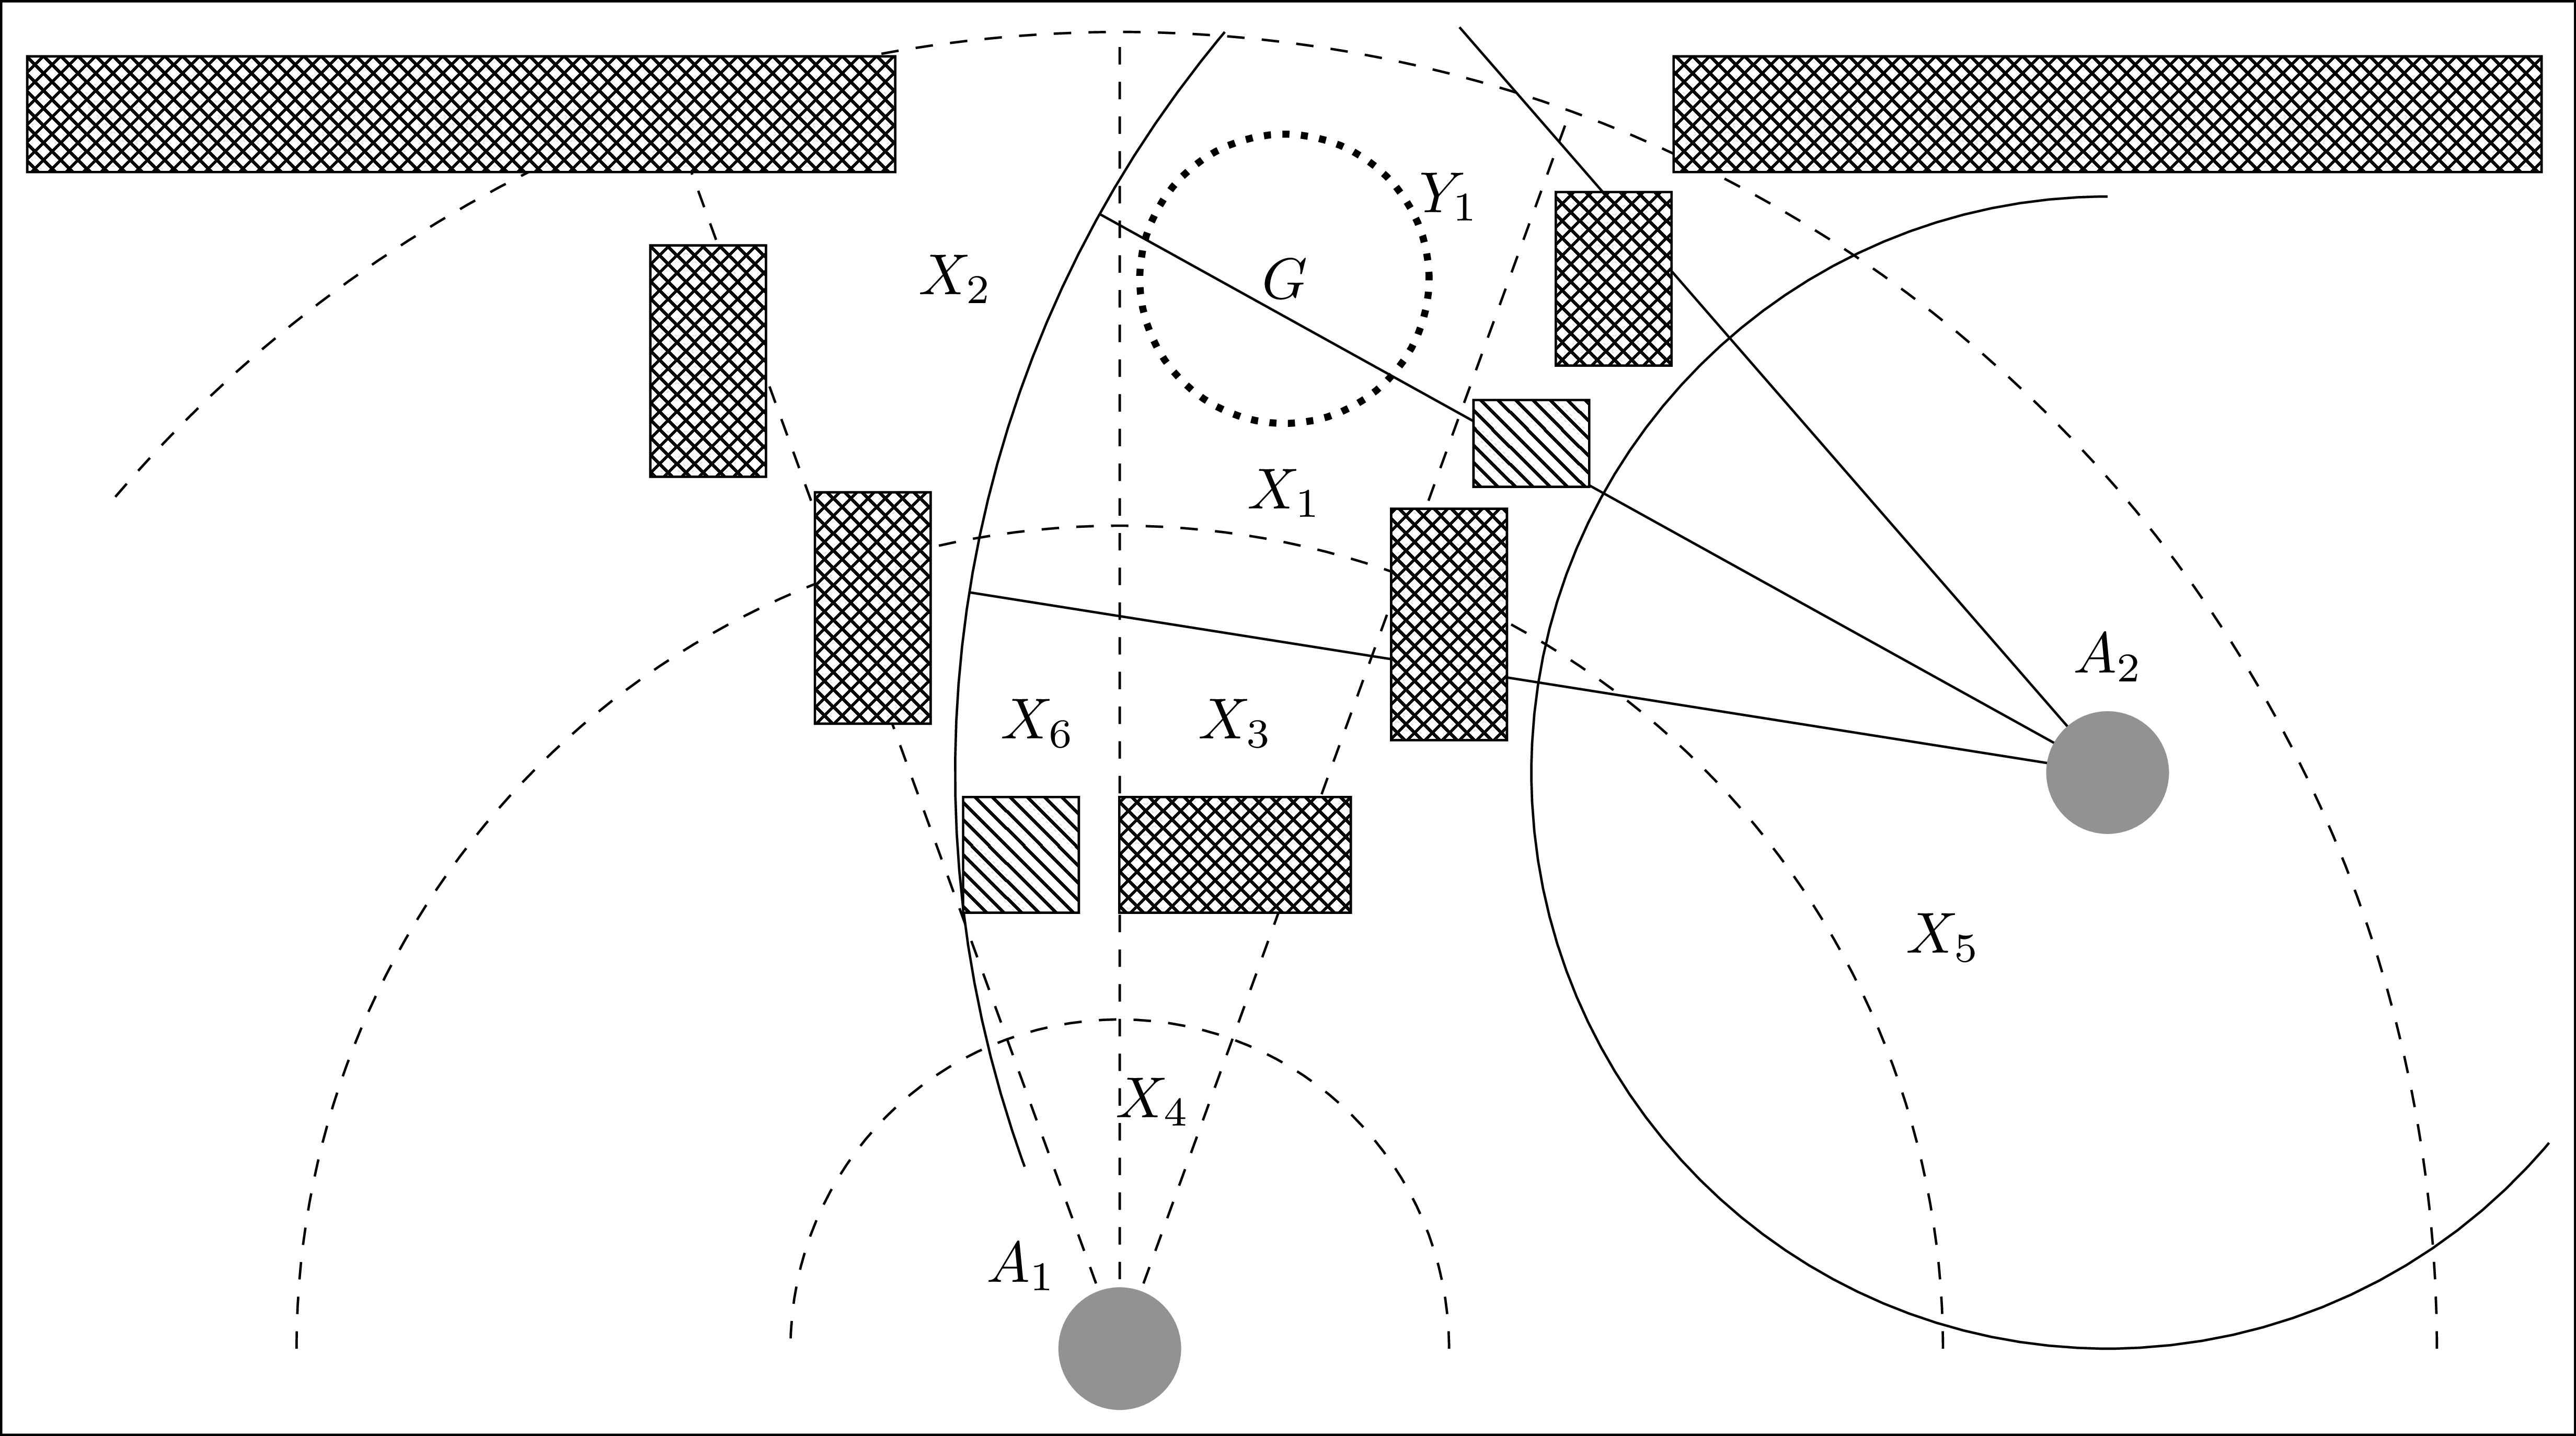
\includegraphics[width=\textwidth]{examples/rita_ex_proc.png}
		\end{figure}
	\end{frame}
	
	\begin{frame}
		\frametitle{Spatial knowledge representation}
		
		Relocation actions --- signs $s_t$ (features $f_t$, $t$ --- relocation type), with corresponding prediction matrices $Z_t$ consist of 3 columns:
		\[
		z_1=(l_x, I), z_2=(l_y, d_u, E), z_3=(l_y, I, t_v),
		\]
		\begin{itemize}
			\item $l_x$, $l_y$ --- features represented category of distance in a spatial logic (e.g., ``far'', ``closely'' etc.), 
			\item $d_u$ --- features represented category of direction in a spatial logic (e.g., ``left'', ``straight'' etc.), 
			\item $t_v$ --- features represented category of time in temporal logic (e.g., ``soon'', ``not soon'' etc.),
			\item $I$ --- feature of agent presence, 
			\item $E$ --- feature of obstacle absence.
		\end{itemize}
	\end{frame}
	
	\begin{frame}
		\frametitle{Model task}
		\begin{center}
			\scalebox{0.7}{
				\animategraphics{12}{examples/slides_colored}{}{}			
			}
		\end{center}
	\end{frame}

	\begin{frame}
		\frametitle{Conclusions}
		\begin{columns}
			\begin{column}{0.55\textwidth}
				\begin{itemize}
					\item We propose psychologically inspired knowledge representation (sign world model) supported by neurophysiological data
					\item Sign world model is used to construct models of cognitive functions
					\item Sign world model is used in STRL cognitive architecture as an implementation of strategic level of control
				\end{itemize}
			\end{column}
			\begin{column}{0.45\textwidth}
				\centering
				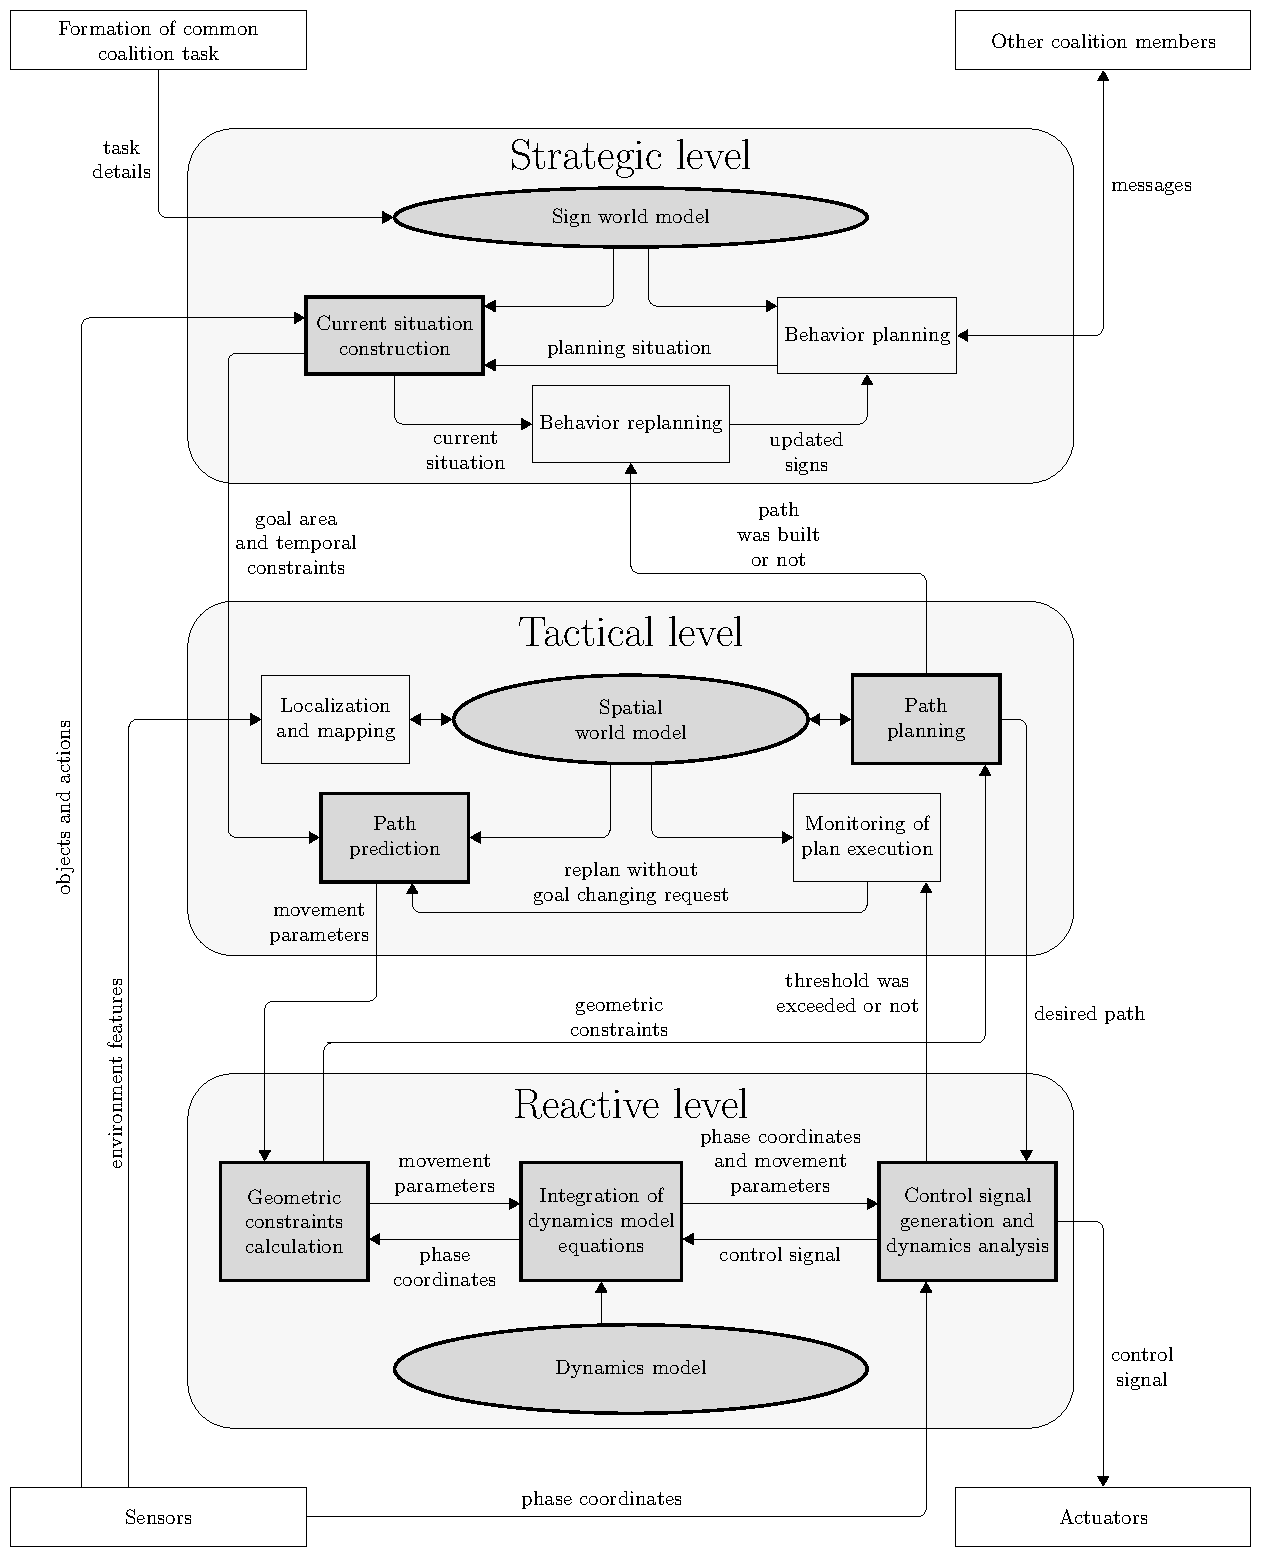
\includegraphics[width=\textwidth]{strl/strl_arch_real_eng}
			\end{column}
		\end{columns}
	\end{frame}
	
	\begin{frame}
		\centering
		\Huge
		Thank you for attention!
		\normalsize
		\par\bigskip
		\par\bigskip
		FRC CSC RAS
		\par\bigskip
		pan@isa.ru
		\par\bigskip
		\url{https://github.com/cog-isa/map-planner.git}
	\end{frame}			
\end{document}
	
	
